\documentclass[a4paper,twoside,phd]{BYUPhys}
% The BYUPhys class is for producing theses and dissertations
% in the BYU Department of Physics and Astronomy.  You can supply
% the following optional arguments in the square brackets to
% specify the thesis type:
%
%   senior  : Produces the senior thesis preliminary pages (default)
%   honors  : Produces the honors thesis preliminary pages
%   masters : Produces the masters thesis preliminary pages
%   phd     : Produces the PhD dissertation preliminary pages
%
% The default format is appropriate for printing, with blank pages
% inserted after the preliminary pages in twoside mode so you can
% send it directly to a two-sided printer. However, for ETD
% submission the blank pages need to be removed from the final output.
% The following option does this for you:
%
%   etd     : Produces a copy with no blank pages in the preliminary section.
%             Remove this option to produce a version with blank pages inserted
%             for easy double sided printing.
%
% The rest of the class options are the same as the regular book class.
% A few to remember:
%
%   oneside : Produces single sided print layout (recommended for theses less than 50 pages)
%   twoside : Produces double sided print layout (the default if you remove oneside)
%
% The BYUPhys class provides the following macros:
%
%   \makepreliminarypages : Makes the preliminary pages
%   \clearemptydoublepage : same as \cleardoublepage but doesn't put page numbers
%                           on blank intervening pages
%   \singlespace          : switch to single spaced lines
%   \doublespace          : switch to double spaced lines
%
% --------------------------- Load Packages ---------------------------------

% The graphicx package allows the inclusion of figures.  Plain LaTeX and
% pdfLaTeX handle graphics differently. The following code checks which one
% you are compiling with, and switches the graphicx package options accordingly.
\usepackage{ifpdf}
\ifpdf
  \usepackage[pdftex]{graphicx}
\else
  \usepackage[dvips]{graphicx}
\fi

%%%%%%%%%%%%%%%%%%%%%%%%%%%%%%%%%%%%%%%%%%%%%%%%%%%%%%%%%%%%%%%%%%
% Edited : Beeshanga
%
% If you need to include any code in the text use this package
% \usepackage{listings}
% It can be used to make key words bold, add colours, etc. Refer
% to http://en.wikibooks.org/wiki/LaTeX/Packages/Listings for
% more information.
%
% For theorems, propositions, proofs and assumtions use this
% package
% \usepackage{amsthm}
% For more information refer to the following website
% http://en.wikibooks.org/wiki/LaTeX/Theorems
%
%%%%%%%%%%%%%%%%%%%%%%%%%%%%%%%%%%%%%%%%%%%%%%%%%%%%%%%%%%%%%%%%%%

% The fancyhdr package allows you to easily customize the page header.
% The settings below produce a nice, well separated header.
\usepackage{fancyhdr}
  \fancyhead{}
  \fancyhead[LO]{\slshape \rightmark}
  \fancyhead[RO,LE]{\textbf{\thepage}}
  \fancyhead[RE]{\slshape \leftmark}
  \fancyfoot{}
  \pagestyle{fancy}
  \renewcommand{\chaptermark}[1]{\markboth{\chaptername \ \thechapter. #1}{}}
  \renewcommand{\sectionmark}[1]{\markright{\thesection \ #1}}


% The cite package cleans up the way citations are handled.  For example, it
% changes the citation [1,2,3,6,7,8,9,10,11] into [1-3,6-11].  If your advisor
% wants superscript citations, use the overcite package instead of the cite package.
\usepackage{cite}
\usepackage{float}
\usepackage{framed}
\usepackage[table]{xcolor}
\usepackage{multirow}



% The makeidx package makes your index for you.  To make an index entry,
% go to the place in the book that should be referenced and type
%  \index{key}
% An index entry labeled "key" (or whatever you type) will then
% be included and point to the correct page.
%\usepackage{makeidx}
%\makeindex

% The url package allows for the nice typesetting of URLs.  Since URLs are often
% long with no spaces, they mess up line wrapping.  The command \url{http://www.physics.byu.edu}
% allows LaTeX to break the url across lines at appropriate places: e.g. http://www.
% physics.byu.edu.  This is helpful if you reference web pages.
\usepackage{url}
\urlstyle{rm}

% If you have a lot of equations, you might be interested in the amstex package.
% It defines a number of environments and macros that are helpful for mathematics.
% We don't do much math in this example, so we haven't used amstex here.
\usepackage{amsmath}
\usepackage{amssymb}
\usepackage{subfigure}
\usepackage{cite}
\usepackage{amsxtra}
\usepackage{amsfonts}
\usepackage{graphicx}
\usepackage{multirow} % This is package for multi-rows in tables added on 7th July 2009 by Arif
%\usepackage{setspace}

% The caption package allows us to change the formatting of figure captions.
% The commands here change to the suggested caption format: single spaced and a bold tag
\usepackage[labelfont=bf,labelsep=colon]{caption}%[2008/04/01]
 \DeclareCaptionFormat{suggested}{\singlespace#1#2#3\par\doublespace}
 \captionsetup{format=suggested}


\usepackage{array}
\usepackage{multirow}
\usepackage{verbatim}
\usepackage{enumerate}
\usepackage{multirow, makecell}


% Defining the symbols

% The hyperref package provides automatic linking and bookmarking for the table
% of contents, index, equation references, and figure references.  It must be
% included for the BYU Physics class to make a properly functioning electronic
% thesis.  It should be the last package loaded if possible.
%
% To include a link in your pdf use \href{URL}{Text to be displayed}.  If your
% display text is the URL, you probably should use the \url{} command discussed
% above.
%
% To add a bookmark in the pdf you can use \pdfbookmark.  You can look up its usage
% in the hyperref package documentation
\usepackage[bookmarksnumbered,pdfpagelabels=true,plainpages=false,colorlinks=true,
            linkcolor=black,citecolor=red,urlcolor=blue]{hyperref}

% ------------------------- Fill in these fields for the preliminary pages ----------------------------
%
% For Senior and honors this is the year and month that you submit the thesis
% For Masters and PhD, this is your graduation date
  \Year{2018}
  \Month{November XX,}
  \Author{Dione Morales}

% If you have a long title, split it between two lines. The \TitleBottom field defines the second line
% A two line title should be an "inverted pyramid" with the top line longer than the bottom.
  \TitleTop{Detecting health misinformation online}
  \TitleBottom{using deep learning methods}
  %\TitleBottom{Line 2 of the Tile} % edited Beeshanga
 \DegreeTitle{Bachelor of Engineering
 \\ Computer Engineering Stream} % edited Beeshanga

% Your research advisor
 \Advisor{Supervisors: Associate Professor Adam Dunn and Dr Rex Di Bona}

% The department undergraduate research coordinator
%  \UgradCoord{A}

% The representative of the department who will approve your thesis (usually the chair)
%  \DepRep{B}

% Acknowledge those who helped and supported you

  \Acknowledgments{
  \vspace{-1.5cm}
    \noindent I would like to acknowledge the countless number of people that have helped me get to where I am today.\newline
    I would also like to thank my supervisors, Rex Di Bona and Adam Dunn, for giving me the freedom and support to be able to work on my current topic. I am deeply grateful for the help and opportunities they have given me.
  }


% The title of the department representative
%  \DepRepTitle{Chair}
  \Statement{
    \noindent I, Dione Morales, declare that this report, submitted as part of the requirement for the award of Bachelor of Engineering in the School of Engineering, Macquarie University, is entirely my own work unless otherwise referenced or acknowledged. This document has not been submitted for qualification or assessment an any academic institution.
    \vspace{0.5cm}

    \noindent     Student's Name: Dione Morales

    \vspace{0.25cm}

    \noindent Student's Signature: Dione Morales (electronic)

    \vspace{0.25cm}

    \noindent     Date: September 9, 2018
    }

% The text of your abstract
\Abstract{
\vspace{-1.5 cm}
With the popularity and ubiquity of social media platforms in today's society, the amount and rate at which information propagates online greatly outnumbers the resources available that can evaluate the quality and credibility of the information that gets shared. This is becoming an increasingly growing issue due to the clickbait model that is commonly adopted by social media platforms and the lack of rigour surrounding the publishing of content online, causing an increase in the number of articles that contain misinformed content. This project aims to investigate the performance of deep learning techniques in evaluating the credibility of information of health-related articles.

}



% Statement of Candidate



\fussy

\begin{document}

 % Start page counting in roman numerals
 \frontmatter

 % This command makes the formal preliminary pages.
 % You can comment it out during the drafting process if you want to save paper.

 \makepreliminarypages


%\clearemptydoublepage
\doublespace
%\include{Publications/publications}

% \clearemptydoublepage
%\include{Organization/organization}

 \clearemptydoublepage
\singlespace
 % Make the table of contents.
 \tableofcontents

\clearemptydoublepage
% Make the list of figures
\listoffigures

\clearemptydoublepage
% Make the list of tables
\listoftables

\clearemptydoublepage

% Start regular page counting at page 1
\mainmatter
%
\chapter{Introduction}
\label{chap:Introduction}

With the popularity and ubiquity of social media platforms in today's society, the amount and rate at which information propagates online greatly outnumbers the resources available that can evaluate the quality and credibility of the information that gets shared. This is becoming an increasingly growing issue due to the clickbait model that is commonly adopted by social media platforms and the lack of rigour surrounding the publishing of content online \cite{Sommariva2018}, causing an increase in the number of articles that contain misinformed content \cite{germanFN} \cite{Vosoughi}.\newline 

The lack of resources that attempt to minimise the spread of misinformation can be attributed to the expert-level knowledge required to determine the credibility of information since a variety of factors such as the actual information, information sources, conflicts of interest and writing style of the article must be evaluated to be able to determine its quality and credibility. This issue is further exacerbated in specific domains such as for health-related content, as the spread of misinformation can have a detrimental effect on people and their communities that don't have access to these kinds of limited resources. \newline

Thus, by developing a method that is capable of automatically assessing the quality and credibility of an article - various methods that intervene between an article and a user can then be developed to minimise the spread and effects of misinformation as the reliance on expert-level knowledge is no longer present.

\section{Project Overview}
\label{sec:ProjectOverview}
This section details the scope of the project and its associated outcomes outlining the various tasks that must be accomplished to successfully complete the project.

One of the key components required to minimise the propagation of misinformation online is to have the ability of automatically evaluating and quantifying the credibility of articles. However, traditional automated methods - such as machine learning-based techniques, still require the domain knowledge of experts to be able to develop the features required by the model. Thus, this project aims to investigate the performance of Deep Learning-based (DL) techniques in evaluating the credibility of information within domain-specific articles via the classification of set criteria that have deemed to be highly correlated with articles that have low credibility. Specifically, this project will focus on evaluating the credibility of online health articles related to vaccination due to the commonly misinformed and controversial views associated with its effects \cite{Burgess2006}. \newline

\section{Motivation}
\label{sec:Motivation}
The propagation of misinformed content can cause people within specific communities to adopt beliefs and practices that can have harmful effects to themselves and also to the people around them. In the context of health-related content specifically, these beliefs and practices can take form in the misuse or mistreatment of medicine or illnesses. A popular example where this issue has emerged is with the misinformed views by certain communities on the ramifications of vaccinating children. \newline

The effects of vaccination and their relation to causing autism within children is a popular example where the belief of inaccurate facts has had a detrimental effect to specific communities and their surrounding environments. The measles outbreak in Minnesota which occurred in April 2017 is a specific case where the misinformed views on the effects of vaccination caused people within a Somali-American community located in the United States to forego the vaccination of their children causing an outbreak of measles, a disease which was declared to be eliminated from the United States in the year 2000 \cite{Hall2017}. Within this specific instance, it was determined that the outbreak of measles was caused by a decline in the coverage of vaccination due to concerns of its effects in relation to the causation of autism. This can be seen in the decreasing trend of the percentage for 24 month-old children that received the measles-mumps-rubella vaccine which fell to a low of 40\% in 2014 where it was at a 90\% high 10 years prior.

\section{Aims}
\label{sec:Aims}

With the primary objective of this project being the evaluation on the effectiveness of deep learning models in determining the credibility of online vaccine-related health articles. Due to the complexity of this project, a set of activities - divided into main goals and stretch goals, have been defined to ensure that the completion of this project remains feasible in the given time frame. The completion of all activities categorized as main goals will signal the realization of the primary objective and the completion of the project. Stretch goals are activities of interest that have been identified as non-essential to the completion of the primary objective but will be worked on after the completion of the project.

\subsubsection{Main Goals}
\label{sec:MainGoals}
\begin{itemize}
	\item Implement and evaluate the performance of machine learning methods for assessing the quality and credibility of vaccine-related text.
	\item Implement a deep neural network method to assess the quality and credibility of vaccine-related text and compare the performance with the previous approaches.
\end{itemize}

\subsubsection{Stretch Goals}
\label{sec:StretchGoals}
\begin{itemize}
	\item Evaluate the effect of transfer learning methods on the training time and performance of the proposed deep neural network method.
\end{itemize}


\chapter{Background and Related Work}
\label{chap:LitReview}

A literature review has been conducted to develop an understanding on the research that has been done in the assessment of the credibility of information, specifically in the context of information related to health and the limitations and capabilities of machine learning techniques and how it differs from deep learning-based methods for the task of document classification. 

\section{Assessing the Quality and Credibility of Health Information}
\label{sec:AssessingInformation}

To have the capability of automating the process of evaluating the quality or credibility of online information, a definition that outlines of what is required by an article to be considered as a credible source of information must be developed. While there has been a significant amount of research that has been done on the development of tools and frameworks that aim to assess the credibility of online health information, there is currently no standardized method or benchmark that is universally used. Tools and frameworks that have been identified to be applicable in the context of this project are: DISCERN \cite{DISCERN}, HealthNewsReview \cite{HealthNewsReview} and Quality Index for health-related Media Reports (QIMR) \cite{QIMR}.

\subsection{Checklists and Criteria}
\label{sec:Checklists}

\subsubsection{DISCERN}
\label{sec:DISCERN}

DISCERN \cite{DISCERN} is a questionnaire designed to assess the reliability of a publication, it consists of 16 questions each with a Likert scale, ranging from 1 (no) to 5 (yes) and is divided into 3 sections. The first section (questions 1 - 8) investigate the reliability of the information and is comprised of questions such as `Are the aims clear?', `Is it balanced and unbiased?' and `Does it refer to areas of uncertainty?'. The second section (questions 9 - 15) assesses the quality of information provided by the publication for treatment choices and is composed of questions such as `Does it describe the risks/benefits of each treatment?' and `Does it provide support for shared decision-making?'. The final section (question 16) assesses the overall rating of the publication (`Based on the answers to all of the above questions, rate the overall quality of the publication as a source of information about treatment choices').


\subsubsection{HealthNewsReview}
\label{sec:HealthNewsReview}

HealthNewsReview \cite{HealthNewsReview} provides a set of 10 criteria designed to act as a framework for evaluating the credibility of health-related media. The criteria is based on the various elements that all health-related media should consist of, the criteria is composed of criterion such as `Does the story compare the new approach with existing alternatives?', `Does the story use independent sources and identify conflicts of interest?' and `Does the story appear to rely solely or largely on a news release?'.

\subsubsection{QIMR}
\label{sec:QIMR}

QIMR \cite{QIMR} is a tool developed to monitor the quality of health research reports presented in the media. The tool considers 5 main factors that have been deemed to be correlated with the quality of research reports based on interviews with health journalists and researchers. The 5 main factors are: background information provided, sources of information used, manner in which results were analysed, context of the research and the validity of their methodology.

\subsection{Studies Applying Checklists to Health Information Online}
\label{sec:ChecklistStudies}

There has been an extensive amount of research conducted which aimed to assess the quality of content for various health-related domains using one of the aforementioned tools \cite{CanteyBanasiak2017} \cite{Cipriani} \cite{Kaicker2010} \cite{Som2012}. A factor shared by these commonly performed studies however, is the use of experts to leverage the tool in assessing the quality and credibility of the information, indicating that commonly used tools such as DISCERN is designed to be used by domain experts in order to produce reliable and consistent results. This sentiment is shared by Batchelor et al. \cite{Batchelor2009} who evaluated performance of the DISCERN tool when used by health professionals and patients. Due to the resource intensive nature of expertly performing this task, the number of articles evaluated, among the various studies examined have been limited ranging between 10 - 300 information sources. This highlights the issue that these tools are not designed to be capable of evaluating the quality and credibility of articles at the scale and speed required to match the pace of online activity and thus must be adapted for the automation of this process. While there has been work in adapting criteria to better encompass the factors that are correlated to the quality and credibility of information within a specific context, such as by Matsoukas et al. \cite{Matsoukas2008}, who expanded the DISCERN tool to improve its capability in assessing the quality of online information, there has not been any published work found that aims to adapt these tools to provide the capability of autonomously assessing the quality and credibility of resources.

\section{Document Classification Methods}
\label{sec:DocumentClassification}

The task of document classification is a heavily researched topic due to its wide number of applications in various domains. Formally, document classification is defined to be the task of finding a classifier $f: D \rightarrow L$ where $D = \{d_1, d_2, \dots, d_n\} $ is a collection of documents and $L = \{l_1, l_2,\dots, l_k\}$ is the set of possible labels that a document $d$ can be classified as. 
\begin{equation}
\label{eq:TextClassification}
f: D \rightarrow L \text{ where } f(d) = l
\end{equation}
Common applications of document classification algorithms are: organization and filtering of news articles, document retrieval, opinion mining, email classification and spam filtering \cite{Aggarwal2012}.

Traditional machine learning-based approaches for document classification, such as Naive Bayes, Support Vector Machines (SVM) and Random Forests, require the manual extraction of features \cite{Aggarwal2012} \cite{Allahyari2017} \cite{Korde2012} \cite{Pasupa2016} as they are incapable of performing feature learning \cite{Basheer2000}. These features are typically either hand-crafted and domain specific, requiring expert-level knowledge for the task domain \cite{Pasupa2016} or are simple and general but prone to the loss of information (e.g. being unable to account for context) since these features, such as term frequency-inverse document frequency (TF-IDF) scores or bag of words (BoW) models, are unable to represent and account for the sequential nature of text.

\subsection{Representing Text as Features}
\label{sec:TextRepresentations}

Due to the unstructured nature of natural text, it is common practice for natural language processing (NLP) tasks to transform the text into a structured representation that minimises the loss of information stored within the original text whilst allowing the model to learn and analyse the features associated with the classification task. However, despite traditional representation methods such as count-based approaches (e.g. TF-IDF) or probabilistic-based approaches (e.g. N-Grams) showing respectable performances in the classification of texts \cite{Zhang} \cite{Zhou2015}, these representations are typically sparsely distributed and have a high dimensionality that scales with the vocabulary size, has difficulty in generalising over unfamiliar information or writing styles \cite{Rosenfeld2000} as the texts are represented using simple mechanisms that are unable to represent high-level information such as context or the semantic relationship of words. Due to the high dimensionality and sparseness of these features, they are computationally intensive to calculate and can require a relatively larger amount of space for storage.\newline

Word embeddings are a more sophisticated language model that overcome these limitations as they are created by learning word vectors through the optimisation for a different task e.g. the prediction of a word based on its context. Through this, the learned embeddings are able to store information such as the similarity of different contexts, syntactic and semantic information within the text and analogies. These embeddings are relatively more efficient and require less time to compute due to their smaller dimensionality. Whilst these embeddings are able to be created using shallow neural networks, deep learning-based models for NLP tasks utilise these embeddings which can also be at the character, phrase or sentence levels \cite{Young}. Word embeddings, such as Word2Vec or GloVe, have produced state-of-the-art results in not only classification tasks \cite{Howard2018} but also for a wide range of NLP tasks such as image annotation \cite{Weston} and sentiment analysis \cite{Cambria2017}, which used the popular word2vec embedding proposed by Mikolov et al. \cite{Mikolov}


\subsection{Machine Learning Methods for Document Classification}
\label{MLDocumentClassificaiton}

\subsubsection{Naive Bayes Classifier}
\label{sec:NaiveBayes}

Naive Bayes is a probabilistic classifier that functions on an assumption in how the data (i.e. the words in a document) is generated. The assumption that these Bayesian classifiers are based on is that the distribution of different words within a corpus are independent from each other. Despite this assumption clearly being wrong when considering the distribution of words within a document (due to the sequential nature of text), Naive Bayes classifiers are still able to perform well in document classification tasks such as the filtering of spam emails \cite{Sahami}.

Naive Bayes classifiers utilize Bayes' theorem, which attempts to find the probability of an event $B$ occurring given some prior condition $A$ i.e. $P(B| A)$. In the context of document classification, Naive Bayes classifiers classifies a document $d$ by calculating the probabilities that the document belongs for all labels $l_i \in L$ and then selecting the highest probability \cite{Allahyari2017}:
\begin{equation}
P(L = l_i| d) = \frac{P(l_i)P(d| l_i)}{P(d)}
\end{equation}

According to Aggarwal et al. \cite{Aggarwal2012}, there are two main types of Naive Bayes classifiers that are commonly used, they are the multivariate Bernoulli model and the multinomial model. The main discriminating factor between these two models is that the Bernoulli model does not take into account the frequency of words as it represents a document using a vector of binary features which signify the presence or absence of words, based on some vocabulary, for a given document. This is in contrast with the multinomial model, which accounts for the frequency of words as the document is represented using a BoW model. Deciding on which model to use for document classification largely depends on the size of the vocabulary as, according to McCallum et al. \cite{McCallum1998}, the multinomial models almost always outperforms the Bernoulli models if the size of the vocabulary is large ($> 1000$) or even if the size has been optimally chosen for both models.

\subsubsection{Support Vector Machines}
\label{sec:SVM}

SVMs are a type of supervised machine learning-based binary classifiers that are extensively used for document classification due to their capability of handling the high dimensional and sparse nature of the common techniques used to represent text documents \cite{Informatik1997}. SVMs are able to classify a document by using a hyperplane to separate the different classes into separate regions. The hyperplane used is determined by choosing the one that maximises the margin of separation (i.e. The Euclidean distance between the hyperplane and all data points in the representation space) between the two classes \cite{Aggarwal2012}.

Consider the illustration shown in Figure \ref{fig:SVMExample} that presents three  two-dimensional hyperplanes, $A$, $B$ and $C$, which separates the classes 'x' and 'o'. Visually, we can determine that $A$ is the hyperplane that maximises the margin of separation, thus, $A$ will be used as the decision rule to classify any new article based on its location in the representation space with respect to $A$. Mathematically, determining which hyperplane to use as the decision rule is an optimisation problem that attempts to maximise the margin represented as shown in Equation \ref{eq:MaxSVM} but is often re-framed to the minimisation of Equation \ref{eq:MinSVM}:

\begin{equation}
\text{maximise: } \frac{1}{2}||\frac{1}{w}||^2
\label{eq:MaxSVM}
\end{equation}

\begin{equation}
\text{minimise: } \frac{1}{2}||w||^2
\label{eq:MinSVM}
\end{equation}


\begin{figure}[H]
	\centering
	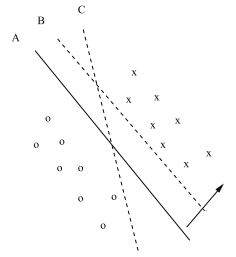
\includegraphics[totalheight=7cm]{images/svm-example.png}
	\caption{Determining the optimal hyperplane \cite{Aggarwal2012}}
	\label{fig:SVMExample}
\end{figure}

This technique of determining the hyperplane requires that the two classes are linearly separable. In situations where this isn't true, the kernel trick \cite{aizerman67theoretical} is applied which is essentially a function that maps data in a particular representation space to another representation space of a different dimension. This change in dimensionality can allow the classes to become linearly separable and thus a hyperplane can then be constructed that separates each class as illustrated in Figure \ref{fig:KernelTrick}.

\begin{figure}[H]
	\centering
	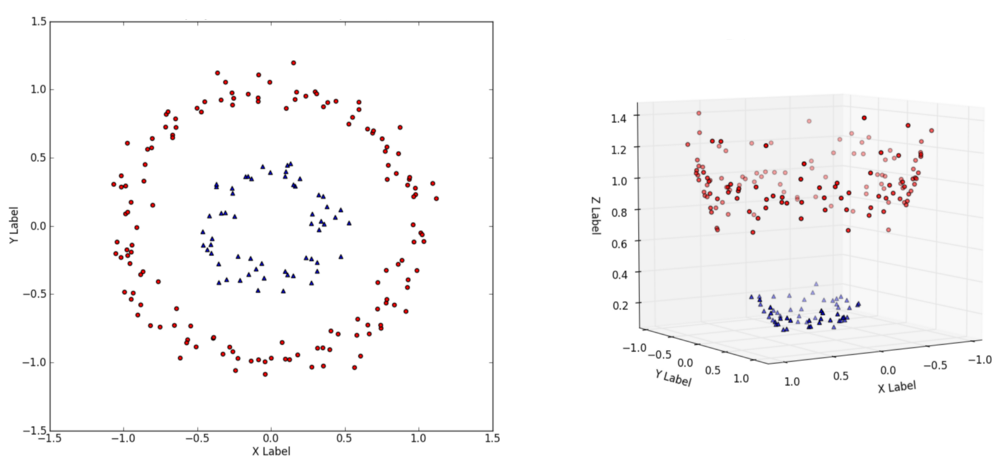
\includegraphics[totalheight=7cm]{images/kernel-trick.png}
	\caption{(Left) Non-linearly distributed data of two classes in a 2D representation space. \newline
		(Right) Linearly separable data of the same classes in a 3D representation space after the application of a kernel function \cite{UnderstandingKernel}.}
	\label{fig:KernelTrick}
\end{figure}

\subsection{Deep Learning Methods for Document Classification}
\label{sec:DLDocumentClassification}

Deep learning models are a class of machine learning models that have the capability of automatically learning a hierarchical representation of data \cite{Basheer2000}. These hierarchical representations are constructed through the use of artificial neural networks, the main underlying mechanism of deep learning models. The most commonly used models for document classification are Recurrent Neural Networks (RNNs), Long Short-Term Memory Networks (LSTMs) - a variant of RNNs and Convolutional Neural Networks (CNNs). \newline

For the task of text classification, there are commonly used, open datasets for specific classification tasks that aim to provide a benchmark in which the performance of different implementations can be compared and to facilitate the data needs of deep learning models. 

\subsubsection{Recurrent Neural Networks}
\label{sec:RNN}

RNNs and LSTMs are commonly used for document classification, or NLP tasks in general, due to their ability to create language models that are able to capture the context and relationships of words within documents over long distances and represent this information at a much more sophisticated level when compared to traditional language models such as TF-IDF or n-grams \cite{Young}. \newline
 
RNNs have had widespread use in solving NLP-related tasks due to their ability in capturing the sequential nature of text at the character, word or sentence level. Consequently, RNNs are capable of creating language models that account for the semantic meaning of words based on the previously occurring words in the sentence, allowing models to be capable of understanding the difference between similar words or phrases (e.g. that the word `dog' is likely referring to the animal whereas `hot dog' would be more likely to refer to food). Accounting for RNNs' capability in handling variable length inputs (e.g. long sentences, paragraphs or documents), they have shown to produce state-of-the-art results in classification tasks such as sentiment, question and topic classification \cite{Howard2018}.\newline

The simplest form of an RNN, as illustrated in Figure \ref{fig:RNN}, consists of three layers: the input layer $x_t$, hidden state $s_t$ and the output layer $o_t$, where $t$ represents the current timestep. The input layer is typically represented as a one-hot encoding or embedding, the output layer is the resulting output which can take many forms, most commonly, it is the output of the softmax function and the hidden state is essentially the memory of the network as it captures and incorporates the information from previous timesteps into the current one. The hidden state is calculated by evaluating Equation \ref{eq:HiddenState}:

\begin{equation}
s_t = f(Ux_t + Ws_{t-1})
\label{eq:HiddenState}
\end{equation}

\begin{figure}[H]
	\centering
	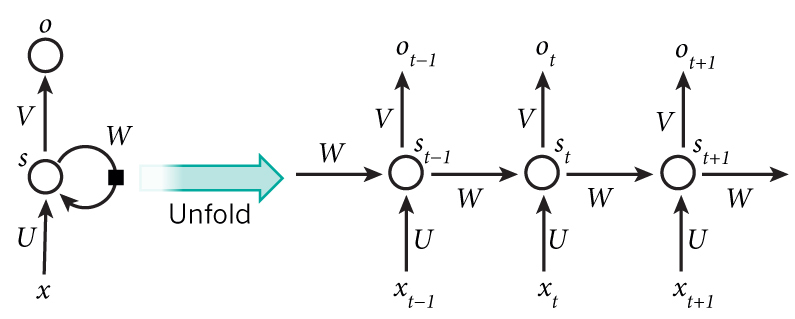
\includegraphics[totalheight=6cm]{images/RNN.jpg}
	\caption{Layout of a simple RNN \cite{RNNDiagram}}
	\label{fig:RNN}
\end{figure}

Where $f$ is a nonlinear function e.g. Rectifier Linear Unit (ReLU), $U$, $V$ and $W$ are weight matrices that are shared across timesteps \cite{Young}. \newline

LSTMs \cite{Hochreiter1997} are a variant of RNNs that improves on it by introducing a 'forget' gate which regulates a cell's state within the network as it can allow information from different cells to be removed or added. This addition allows LSTMs to overcome the vanishing and exploding gradient problem \cite{Socher} that feedforward networks i.e. RNNs are prone to.

\subsubsection{Convolutional Neural Networks}
\label{sec:CNN}

Despite CNNs being initially developed for object recognition tasks \cite{LeCun1999}, they are commonly employed for text classification tasks such as sentence classification and sentiment analysis as they have shown to produce competitive results when compared to RNNs and LSTMs \cite{Collobert2011} \cite{Kim} \cite{Nogueira}. \newline

In the context of text classification, a typical CNN is composed of the following main elements \cite{Young}:

\begin{itemize}
	\item Kernels - Convolutional filters that acts as a sliding window function through an embedding matrix. CNNs typically employ hundreds of kernels each of which learns to extract for specific n-gram pattern.
	\item Pooling layer - Commonly either a max or average pooling layer, which maps the input to a fixed dimension in order to reduce the dimensionality of the output and ensuring that the most salient n-gram features of a sentence is kept.
	\item Nonlinear activation function - Such as a ReLU function applied to the results to output a prediction.
\end{itemize}

By stacking the kernels and pooling layers, deep CNNs can be constructed which can automatically capture an abstract and rich representation of the information \cite{Young}. These representations are considered to be efficient when compared to traditional representation methods (e.g. n-grams) as they don't require the storage of the entire vocabulary and is not as computationally intensive. CNNs are also more computationally efficient when compared to RNNs and LSTMs, CNNs typically require larger amounts of data in order to produce competitive results against its RNN and LSTM counterparts due to the higher number of trainable parameters that CNNs have. Another limitation of CNNs is their inability to model long-distance relationships and preserving the sequential nature of text within its representations.

\subsection{Classifying Documents with Limited Labelled Examples}
\label{sec:TransferLearning}
Typically, large amounts of training data is required to train a deep learning model in learning the language model for state of the art results, in the task of document classification for instance, the size of commonly used non-domain specific datasets range from hundreds of thousands of training examples to millions \cite{Conneau2017} \cite{Zhang}. For situations where you are required to procure a completely new dataset, such as training a deep learning model for a non-standard text classification task, it can be unfeasible  or not worthwhile to invest the time and resources in creating the dataset. 

\subsubsection{Transfer Learning}
\label{sec:TransferLearningReview}

Transfer learning involves the repurposing of an already existing deep learning model that has been trained to perform a different, but similar, task using an already existing and available dataset. It functions on the idea that the features automatically learned by a model for some similar task is general enough such that they can then be utilised on the completely new task. 

Howard et al. \cite{Howard2018} has proposed a transfer learning methodology for text classification which was designed to be able to develop models with state-of-the-art results for tasks where there is a limited amount of training data available. \newline

The proposed method involves the use of an inductive learning technique \cite{Pan2009}:
\begin{enumerate}
	\item Create a language model to capture general features of the language by training on a general-domain corpus (e.g. wikitext103 \cite{Merity2016}).
	\item Learn task specific features by fine-tuning the language model using the target task data.
	\item Adapt the high-level representations of the classifier that uses the language model, while preserving the low-level representations, using gradual unfreezing \cite{Howard2018}
\end{enumerate}

Whilst transfer learning is useful to train models for non-standard tasks where access to data is limited, it is also an optimisation technique, using previously acquired knowledge, to save time or improve model performance \cite{Pan2009}. This potential performance improvement is illustrated in Figure \ref{fig:TransferLearning} and is also demonstrated by Howard et al. \cite{Howard2018} for common text classification tasks such as question, topic  classification and sentiment analysis.

\begin{figure}[H]
	\centering
	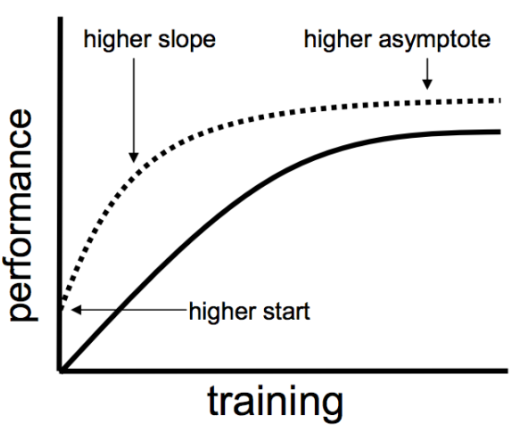
\includegraphics[totalheight=7cm]{images/transfer-learning.png}
	\caption{Potential improvements in performance using transfer learning \cite{Browniee2017}}
	\label{fig:TransferLearning}
\end{figure}


\section{Scaling the Assessment of Quality and Credibility of Health Information}
\label{sec:ScalingAssessment}

The limited amount of articles that were evaluated was a common theme among the studies that aim to assess the credibility and quality of information \cite{Batchelor2009} \cite{CanteyBanasiak2017} \cite{Cipriani} \cite{Kaicker2010} \cite{Som2012}.
This makes evaluating the credibility of online articles impractical when using the existing assessment tools as described in Section \ref{sec:Checklists}, due to the persistence, pace and volume of the production and propagation of online content. Due to the capabilities of machine learning models, they can be leveraged to accomplish the task of automatically assessing the credibility of online articles on a large scale as models, such as deep learning models, have shown the ability to develop high-level representations of language which can then be leveraged to be able to differentiate between credible and misinformed articles.


\chapter{Methods}
\label{chap:Methods}

\section{Approach}
\label{sec:Approach}

Through a review of the relevant literature, I found that there is value in being able to appraise the credibility of online health information for use in tools that could help limit the spread of misinformation. However, it is a challenge to apply credibility appraisal tools at scale because the process is time-consuming and often requires a certain level of expertise to use. Tools for automating this task are therefore likely to be of value but to date most research in the area simply aims to label fake news or uses heuristics to identify misinformation available online. In this chapter, I describe the approach I used to address this challenge using machine learning to train classifiers capable of predicting whether an online article meets a set of credibility criteria.\newline

This involved obtaining training and testing data consisting of online vaccine-related articles along with its associated credibility that were manually determined by a team of health professionals using a pre-existing framework (Section \ref{sec:StudyData}). \newline

Once the dataset was created, a set of machine learning and deep learning models were implemented (Section \ref{sec:SystemModel}). The machine learning models comprised of the implementation of widely used text classifiers, Naive Bayes (NB) and Support Vector Machines (SVMs), in combination with a variety of textual representation methods. The deep learning model involved the construction of a Quasi-Recurrent Neural Network (QRNN) in conjunction with a fine-tuned language model (LM). \newline

The models are then analysed and evaluated on their feasibility for real-world use based on their ability to correctly predict the label for each criteria and other factors such as the training time of the models and their storage requirements (Section \ref{sec:Experiments}).

\section{Study Data}
\label{sec:StudyData}

\subsection{Dataset}
\label{sec:Dataset}

I obtained a set of vaccine-related online articles via the URLs included in a set of 6.59 million Twitter posts (tweets) from 1.86 million Twitter users collected between January 2017 and March 2018. There were 1.27 million unique URLs included in the set of tweets. A majority of the URLs led to web pages that could not be used as they were either broken or were links to other social media posts and YouTube videos. After removing web pages that could not be used in the analysis, I finally included a set of 3,348 vaccine-related online articles (the corpus). The content of the set of online articles included in the corpus ranged from descriptions of recent research to discussions (Figure \ref{fig:ArticleExample}). \newline

\begin{figure}
	\begin{framed}
	\begin{quotation}
		Thousands of parents describe their children as ‘fine’ one day, then their children suddenly develop autism (a neurological regression) after vaccines.\newline
		
		What does the science say? It agrees... \newline
				
		But first let’s go through the numbers. The increase in autism cases in the last three decades is truly shocking. Before the 1980s, autism was so rare, it was not even tracked. Remember the eye-opening movie RainMan with Dustin Hoffman? Before that movie came out in the early 1980s, many had no idea what autism was.\newline
		
		At that time, statistics put the rate of autism at 1 in every 8,000 children. By the mid-1990s, it was around 1 in 1000 children, but by the mid-2000s, it had risen to 1 in 250. The epidemic has continued and in 2017, the US National Center for Health Statistics just released the latest rate: 1 in every 36 children now have autism (link to report here). These skyrocketing rates clearly prove there is a true epidemic of autism in the United States.\newline
		
		So what is autism? Autism is brain damage caused by brain inflammation, which can be triggered by the heavy metals used as adjuvants (aka ingredients) in vaccines. Just as thousands of parents saw firsthand with their own children. Read some of these stories here.\newline
		
		Doctors usually try to deny any responsibility and connection to the vaccines they gave by saying “Autism is genetic.” But autism is even listed as a possible reaction (or side effect) of vaccines on some of the vaccine inserts. Unfortunately, doctors rarely see these inserts, favoring the pharmaceutical marketing sheets over real science.\newline
		
		So let’s get to that real science — the type that is NOT funded by the pharmaceutical industry that wants to sell vaccines and then the prescription drugs that these children are on to control the symptoms of autism, an issue possibly caused by the vaccines.\newline
		
		
	\end{quotation}
	\end{framed}
	\caption{Excerpt from a low credibility vaccine-related online article \cite{AutismVaccine}.}
	\label{fig:ArticleExample}
\end{figure}

The articles included in the corpus were collected by selectively accessing the extracted URLs embedded within tweets that contained specific keywords related to vaccination on Twitter. This was done to ensure that the articles used represented, to some degree, the articles that are most likely to contribute to the effects of the propagation of misinformation as the articles that have been collected and labelled are the ones being shared and discussed online. \newline




\subsection{Credibility Criteria and Appraisal}
\label{sec:CredibilityCriteria}
The credibility criteria were developed by a team of three researchers from the Centre for Health Informatics as part of a separate project funded by the National Health \& Medical Research Council. The seven criteria describe a set of desirable characteristics for online health information (Table \ref{table:Criteria}). The development of the criteria was based on a set of existing tools and checklists (see Section 2.1), which was adapted by the researchers to be applicable to online articles about vaccination. \newline

Prior to creating the dataset for this project, a small pilot experiment was conducted by the team that developed the criteria to ensure that the simplicity and objectivity of each criteria allowed for consistent and reliable labels to be produced. In the pilot test of the credibility criteria, each of the three researchers manually and independently labelled the same set of 30 online articles. The team then measured how well their answers matched, resolving differences by discussion, and updating the definitions of the criteria to improve the consistency. \newline


The final tool used by the three investigators included seven criteria, which were inspired and derived from existing checklist-based tools and designed specifically for use with vaccine-related online articles (Table 3.1). They then used the tool to manually assess an additional 470 articles; for each article, the investigators labelled whether the article satisfied each of the individual criteria. Once labelled, the article's credibility was then aggregated to a credibility score which is defined by the number of criteria that were satisfied. Due to the infeasibility of developing the expert-level knowledge and skill set required to manually label the articles given the time constraints of this project, I did not participate in this labelling process.\newline


When sampling articles, we expected to find relatively few high credibility articles, so the team over-sampled from the subset of articles that were directly linked to research literature. To do this, we used Altmetric, an organisation that provides access to information about how often research articles are mentioned in online media. As a consequence, the proportion of online articles that met the first criterion (identifying the source of evidence) was higher than might be expected from a random sample (Figure \ref{fig:LabelDistribution}). Relatively few articles satisfied criterion 3 or criterion 7, while most articles satisfied criterion 4 and criterion 6. Overall, the resulting data were relatively unbalanced, which has implications in relation to the training of classifiers, as discussed in Chapter \ref{chap:Results}.


\begin{figure}[H]
	\centering
	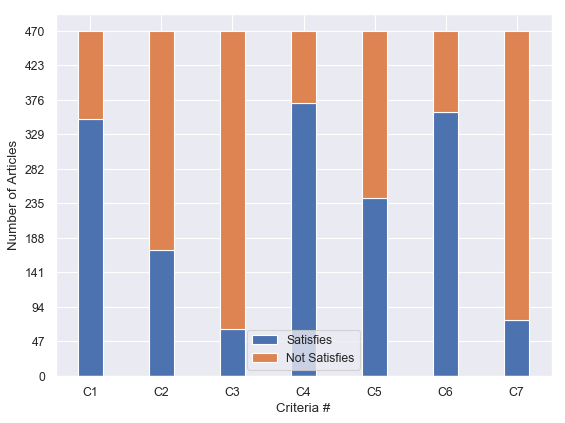
\includegraphics[totalheight=7cm]{images/label-distribution.png}
	\caption{Distribution of labels amongst the expert-labelled articles.}
	\label{fig:LabelDistribution}
\end{figure}


I then aggregated the total number of criteria met by an aritcle to produce a credibility score for each of the 470 documents, which produces a score that may take any integer value between 0 and 7. Partly because of the way the online articles were sampled for expert labelling, the credibility scores for the expert-labelled set were unevenly distributed. The largest proportion of the expert-labelled articles received a credibility score of 4; only 14 and 4 articles received a credibility score of 0 and 7, respectively (Figure \ref{fig:ArticleDistribution}).

\begin{figure}[!htb]
	\centering
	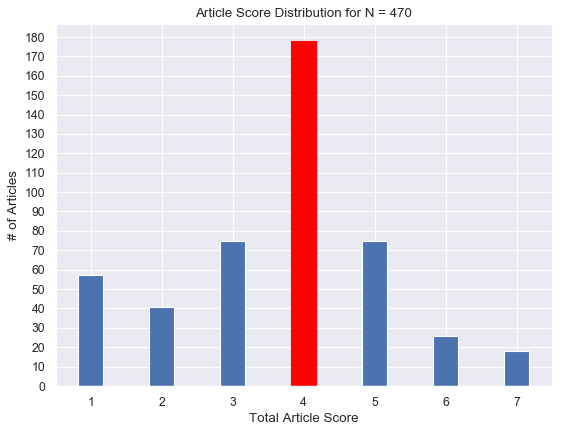
\includegraphics[totalheight=7cm]{images/article-score-distribution.png}
	\caption{Distribution of article scores amongst the expert-labelled articles.}
	\label{fig:ArticleDistribution}
\end{figure}

\begin{table}[H]
	\centering
	\resizebox{\textwidth}{!}{%
	\begin{tabular}{|p{0.3cm}|p{5cm}|p{10cm}|}
		\hline
		\# & Criteria                                                                           & Description                                                                                                                                                                                                                                                                                                                                                             \\
		\hline
		1  & Identifies the information sources supporting a position            & Score 1 if the article clearly indicates what sources of information are used to support its main claims or statements. \\
		\hline
		
		2  & Uses information sources based on objective, scientific research. & Score 1 if the article's main claims are based on objective, scientific research.\newline Score 0 if the article uses anecdotal evidence exclusively to support its main claims.                                                                                                                                                  \\
		\hline
		
		3  & Communicates the strength or weakness of the evidence used to support a position. & Score 1 if the article includes adequate details about the level of evidence offered by the research.                                                                                                                                                                                                                        \\
		\hline
		4  & Does not exaggerate or overstate a position.                         & Score 0 if the article: \newline- Uses unjustified sensational language \newline- Presents information in a sensational, emotive or alarmist way \newline- Selectively or incorrectly presents evidence                                                                                                                                       \\
		\hline
		5  & Presents information in a balanced manner. & Score 1 if the article:\newline- Identifies/acknowledges uncertainties and limitations in the research\newline - Acknowledges where an issue is controversial, and includes all reasonable sides in a fair way\newline - Uses a range of information sources\newline - Provides a balanced description of the strengths and weaknesses of the study
		\\
		\hline
		6  & Uses clear, non-technical language that is easy to understand. & Score 1 if the article:\newline - Is professionally written, with proper grammar, spelling, and composition\newline - Defines any technical jargon, or uses everyday examples to explain the technical terms or concepts                                                                  \\
		\hline
		7  & Is transparent about sponsorship and funding. & Score 1 if the article:\newline - Clearly distinguishes content intended to promote or sell a product from service from educational and scientific content\newline - Discloses sources of funding for the organisation/website
		\\
		\hline                                                                    
	\end{tabular}}
	\caption{Credibility Criteria}
	\label{table:Criteria}
\end{table}



\section{Model Implementation}
\label{sec:SystemModel}

\subsection{Preprocessing}
\label{sec:ModelPreprocessing}

Preprocessing of the unlabelled and expert-labelled articles of the dataset to obtain its raw article text was performed by removing the superfluous content from the web-scraped pages such as the HTML, CSS and JavaScript elements. They were removed as they were deemed to have no contribution to the credibility of the article's content with regards to the credibility criteria. Once the unstructured article text was obtained, it was transformed into a more functional representation via tokenising each article into sentences that consisted of unigrams (Figure \ref{fig:PreprocessingExample}). The steps involved in the preprocessing were designed to produce a standard set of documents that could then be used consistently across each of the approaches to constructing features (detailed in Section 3.3.2).

\begin{figure}[H]

	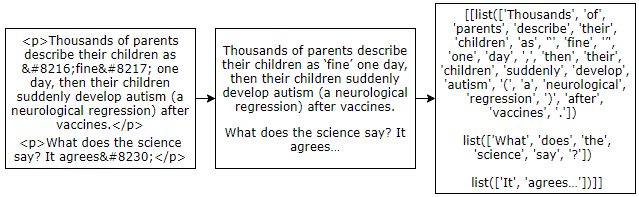
\includegraphics[width=16cm]{images/Preprocessing-example.png}
	\caption{Example process of preprocessing phase showing the original HTML format (left), removal of superfluous content (middle) and the restructuring into a more standardised representation for feature construction (right).}
	\label{fig:PreprocessingExample}
\end{figure}

\subsection{Feature Construction}
\label{sec:ModelFeatureConstruction}

In document classification tasks, the way document text is transformed into a set of features can have a substantial impact on the overall performance. Traditional approaches to feature representation include simple methods that take the words from a corpus and assign values to them; for example, based on the frequency with which they occur in the text. More sophisticated methods are able to transform document text into multi-dimensional vector representations that captures information such as the similarity between words or the context in which a word is used in.



\subsubsection{Bag of Words}
\label{sec:FeatureSelectionBoW}
Two unigram BoW model variants were constructed using the expert-labelled articles; both of which were limited to a maximum of 20,000 n-grams. Identical BoW models were also constructed for different maximum unigram amounts, specifically, BoW models for 5,000 and 10,000 unigrams were also tested. The first BoW model included all of the words that appeared within the articles. The second BoW model was constructed by removing common English stopwords such as 'the', 'is' and 'are' listed in NLTK's English stopwords corpus \cite{Bird2009} were removed.

\subsubsection{Term Frequency - Inverse Document Frequency}
\label{sec:FeatureSelectionTFIDF}
TF-IDF scores of the unigrams extracted from the expert-labelled articles which were limited to the top 20,000 scores were calculated and used for evaluation. Two sets of scores were used for evaluation, the first set of scores was calculated with the inclusion of all words in the expert-labelled articles and the second set of scores was calculated with the removal of stopwords.

\subsubsection{GloVe}
\label{sec:FeatureSelectionGloVe}

A pre-trained global vector (GloVe) \cite{pennington2014glove} was also used for the evaluation of the ML-based models. This was accomplished by using the mean value of each word's vector representation. The GloVe vector used was trained on 6 billion tokens, with a vocabulary size of 400,000 and a has dimensionality of 300.

\subsubsection{Language Models}
\label{sec:FeatureSelectionLM}

A general, non-domain specific language model (LM) was constructed for evaluating the DL-based model. This was achieved by training a Quasi-Recurrent Neural Network (QRNN) using the same hyperparameter settings and training scheme described by Bradbury et al. \cite{bradbury2016quasi} using the Wikitext-103 corpus. Wikitext-103 is a corpus consisting of approximately 28,000 Wikipedia articles that meet either the `Good' or `Featured' article criteria \cite{Merity2016}. \newline

The LM was then fine-tuned using the techniques proposed by Howard et al. \cite{Howard2018} by using the 2,878 unlabelled articles from the corpus in order to learn the task-specific features for classification. The Wikipedia articles used to create the non-domain specific LM also underwent the same preprocessing process described in Section \ref{sec:ModelPreprocessing}, except for the removal of webpage elements, which was unnecessary.

\subsection{Model Construction}
\label{sec:ModelSelection}

In the context of this section, a model refers to the combination of a feature and classifier. The following sections detail the implementation process of the classifiers and the features used in conjunction to create the various models.
For the software used to implement the models, the NB and SVM models were implemented using scikit-learn, an open source machine learning library in Python \cite{scikit-learn}. The QRNN model which utilised the LM and QRNN classifier was implemented using PyTorch \cite{paszke2017automatic} and the open-source software developed by Bradbury et al. \cite{bradbury2016quasi} and Howard et al. \cite{Howard2018}. 

\subsubsection{Naive Bayes}
\label{sec:ModelNB}

A multinomial Naive Bayes (NB) classifier was used for evaluation, based on the reasoning discussed in Section \ref{sec:NaiveBayes}. Along with the 3 types of features (BoW, TF-IDF and GloVe) and their variants (inclusion/exclusion of stopwords) used in conjunction with the NB classifier, a total of 35 NB models (7 criteria $\times$ 5 features evaluated) were developed (Figure \ref{fig:MLModels}). The hyperparameter values were optimised via grid search and evaluated using 10-fold cross-validation. 

\subsubsection{Support Vector Machine}
\label{sec:ModelSVM}

A linear support vector classifier (linear SVC), an SVM with a linear kernel, was used for evaluation. Similar to the implementation of the NB models, a classifier was trained for each criteria with the same set of features totalling 35 SVM models. The hyperparameter values were also optimised and evaluated using grid search and 10-fold cross-validation.

\begin{figure}[H]
	\centering
	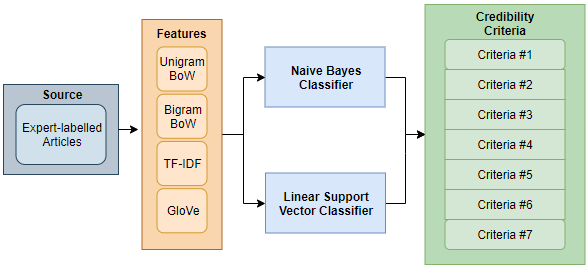
\includegraphics[totalheight=6cm]{images/ml-models.png}
	\caption{Overview of the NB and SVM models implemented.}
	\label{fig:MLModels}
\end{figure}

\subsubsection{Quasi-Recurrent Neural Network}
\label{sec:ModelQRNN}

In addition to using a QRNN for constructing the fine-tuned and general LM, another variant was implemented as a classifier. The architecture for the classifier was adapted from the experiments conducted by Bradbury et al. \cite{bradbury2016quasi} for sentiment classification. From this model, the number of units within each layer was increased to 2500 and the embedding size was changed to 150. The model was trained for up to 20 epochs with a batch size of 100, however the model began to converge after only 5 epochs. In contrast to the NB and SVM models, 21 QRNN models (7 classifier $\times$ 3 LM variants) were created (Figure \ref{fig:DLModels}).

\begin{figure}[H]
	\centering
	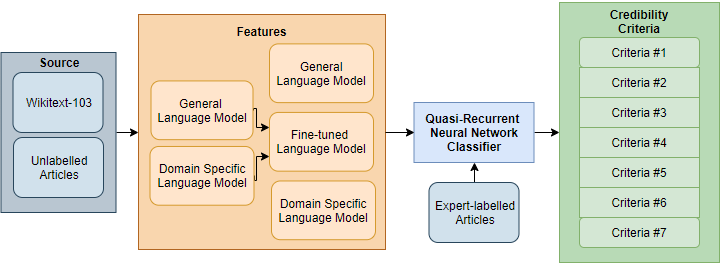
\includegraphics[totalheight=5.6cm]{images/dl-models.png}
	\caption{Overview of the QRNN models implemented.}
	\label{fig:DLModels}
\end{figure}

\section{Experiments}
\label{sec:Experiments}

Considering the context of this project, other factors such as the size of the model and its training speed must be considered in addition to its capability on correctly producing the correct labels to determine the feasibility of deploying the model for a real-world application. 

\subsection{Performance}
\label{sec:PerformanceExperiments}

Two experiments have been conducted to evaluate the performance of a model. The credibility classification experiment is designed to determine the model's ability to produce the correct label on a criteria-level allowing for a more detailed insight on the reasoning for a particular article's credibility score. Whereas the low credibility identification experiment is designed to determine the model's ability to correctly determine whether an article is considered to have low credibility or not for situations where the detailed insight is not required.

\subsubsection{Credibility Classification Experiment}
\label{sec:CredibilityClassificationExperiment}
The credibility classification experiment is a set of binary classification tasks which aims to determine a model's ability in correctly identifying whether an article either satisfies or doesn't satisfy a certain criteria. 
For each criteria, the respective NB and SVM model is employed along with the QRNN model to classify whether the article satisfies the criteria or not. The correctness of the model was then evaluated by measuring the micro averaged f1-scores via 10-fold cross-validation, which is the harmonic mean of the precision and recall of a model's predictions. This experiment attempts to assess the feasibility in providing insight on the factors that attributed to the credibility of an article in addition to identifying the model(s) that best classify a specific criteria.


\subsubsection{Low Credibility Identification Experiment}
\label{sec:LowCredibilityIdentification}
The Low Credibility Identification Experiment was designed to evaluate the capability of a model to identify low credibility articles which have been defined to be articles with a credibility score lower than 3. The expert-labelled articles were then separated into two  classes based on this condition and the best performing model(s), determined from the results of the credibility classification experiment, was then applied and evaluated using the calculated micro averaged f1-scores. \newline

The classification of low credibility articles was then carried out following two methodologies. The first methodology involves the calculation of the article's credibility score via the classification of each criteria, resulting in a total of seven binary classification tasks. The second methodology utilises the separated expert-labelled articles to construct a new binary label consisting of the labels `Credible' for articles that had a credibility score greater than or equal to 3 and a `Not Credible' label for the remaining articles. This method results in only a single binary classification where the model is trained to classify an unseen article as one of the aforementioned labels rather than carrying out the classification of each credibility criteria.

\subsection{Training}
\label{sec:TrainingExperiments}
The training time for a model is another factor that must be considered when determining the feasibility of deploying and using a model on a real-world application. This is because the model will require to be constantly re-trained when additional article samples are incorporated as the model encounters new and never before seen information. To ensure consistent results, Amazon Web Service's EC2 instances \cite{AWS} have been used to act as an isolated environment for timing the training of the NB, SVM, QRNN classifiers and also  the creation of the LM. The reported training times in Section \ref{sec:TrainingTime} are for the best performing NB and SVM-based models, which were trained within a c5.2xlarge instance utilising all CPU cores. The reported training times for the QRNN classifier and LM were obtained using the P3 instances and utilising only a single K80 GPU.


\subsection{Storage}
\label{sec:StorageExperiments}
To minimise the frequency in which a model will have to be re-trained or re-created, storing the model for later use is required. Since the entire implementation was completed using Python, the Python module \textit{pickle} was used to store the models externally. Pickle serialises any Python object into a byte stream allowing a model to be persistently stored. The NB and SVM-based models were stored using pickle and the size of the resulting byte stream was then measured. The QRNN classifier and LM were stored using PyTorch's inbuilt save function, that acts as a wrapper over the \textit{pickle} module which provides storage optimisations for PyTorch objects. The resulting byte stream of the model is then recorded and reported in Section \ref{sec:StorageRequirements}.



\chapter{Results}
\label{chap:Results}

In this chapter I detail the results of the experiments described in the previous chapter. These are the results that come from testing the performance, training time, and storage requirements of the models in the classification task of predicting whether a document extracted from a web page satisfies each of the seven credibility criteria. The classifiers include the proposed QRNN-based deep learning approach as well as classifiers trained using NB and SVM methods.

\section{Performance}
\label{sec:AccuracyResults}
\subsection{Credibility Classification}
\label{sec:CredibilityClassificationResults}


\iffalse
The performance of all 84 models were evaluated via the credibility classification experiment. Divided into the three main groups of models (NB, SVM and QRNN), the NB-based models (Table \ref{table:PerformanceResultsNB}) outperformed the SVM-based (Table \ref{table:PerformanceResultsSVM}) and QRNN-based models (Table \ref{table:PerformanceResultsQRNN}) overall with an aggregated average performance measure of 0.795, followed by SVM-based models with a measure of 0.780 and finally QRNN-based models with a measure of 0.397. Despite the NB-based models having performed better on average, the best performing model for labelling was the SVM-based, SVM + TF-IDF model with the stopwords removed from the article's text. \newline


\fi

I trained and tested the performance of NB and SVM classifiers in combination with two feature representations, BoW and TF-IDF, implementations of which as described in the prior chapter. For each criteria, all combinations of classifiers and feature representations was then trained to perform a binary classification task that aimed to predict whether a given article satisfied that criteria. This produced a combined total of 70 NB-based and SVM-based models. \newline

The performance of the models varied considerably across all criteria (Table \ref{table:PerformanceResultsNBSVM}). When considering both the NB and SVM based approaches, the models had the most difficulty in classifying criteria 6 producing the lowest micro averaged f1-score of 0.71, with the best performing model for this criteria being an SVM classifier paired with TF-IDF (stopwords removed) who achieved a score of 0.77. The models were most successful in labelling criteria 3 which had a micro averaged f1-score of 0.85 with the top performing model being a tie between the NB and SVM classifier paired with BoW (stopwords) with a score of 0.90. \newline

Across all criteria, the SVM with TF-IDF (stopwords removed) was the best-performing of the models, followed by the NB classifier using BoW with stopwords removed. This shows that the removal of stopwords is beneficial in improving model performance which is consistent with other research done for text classification tasks [\textit{cite}]. \newline

The performance of the models may have highly been influenced by the unbalanced nature of the training data as the measured scores are proportionate to the imbalance of the label. This is most evident in the model performance for criteria 3, the most imbalanced label as shown in Figure \ref{fig:LabelDistribution}, where the models had the highest success in classifying. \newline

\begin{table}[H]
	\centering
	\resizebox{\textwidth}{!}{%
		\begin{tabular}{|p{6cm}|p{2.6cm}|p{2.6cm}|p{2.6cm}|p{2.6cm}|p{2.6cm}|p{2.6cm}|}
			
			
			\hline
			
			\textbf{Criteria} &  & \textbf{BoW \newline (all words)  }                                                                       & \textbf{BoW \newline (stopwords removed)} &\textbf{TF-IDF \newline (all words) }& \textbf{TF-IDF \newline (stopwords removed)} & \textbf{GloVe} \\
			\hline
			
			\multirowcell{2}{\textbf{Criteria 1:} \\ \textbf{Use of evidence} } 
			& NB & 0.79 & 0.85 & 0.79 & 0.79 & 0.82 \\ 
			& SVM & 0.82 & 0.78 & 0.80 & \textbf{0.86} & 0.60 \\ 
			\hline
			
			
			\multirowcell{2}{\textbf{Criteria 2:} \\ \textbf{Based on objective research}} & NB & 0.70 & 0.79 & 0.74 & 0.80 & 0.78 \\ 
			& SVM & 0.70 & 0.80 & 0.70 & \textbf{0.85} & 0.77 \\ 
			\hline 
			
			
			\multirowcell{3}{\textbf{Criteria 3:} \\ \textbf{ Explains limitations and} \\ \textbf{uncertainties}} 
			& NB & 0.86 & \textbf{0.90} & 0.87 & 0.89 & 0.89 \\ 
			& SVM & 0.86 & \textbf{0.90} & 0.84 & 0.89 & 0.63 \\ & & & & & & \\ 
			\hline 
			
			
			\multirowcell{3}{\textbf{Criteria 4:} \\ \textbf{No sensationalist or} \\ \textbf{exaggerated language}} 
			& NB & 0.84 & 0.84 & 0.80 & 0.81 & 0.82 \\ 
			& SVM & 0.80 & \textbf{0.87} & 0.84 & 0.86 & 0.61 \\ & & & & & & \\ 
			\hline 
			
			
			\multirowcell{2}{\textbf{Criteria 5:} \\ \textbf{Balanced information}} 
			& NB & 0.79 & \textbf{0.80} & 0.79 & 0.77 & 0.78 \\ 
			& SVM & 0.68 & 0.78 & \textbf{0.80} & \textbf{0.80} & 0.59 \\
			\hline 
			
			
			\multirowcell{2}{\textbf{Criteria 6:} \\ \textbf{Simple Language}} & NB & 0.75 & 0.74 & 0.62 & 0.69 & 0.68 \\ 
			& SVM & 0.75 & 0.72 & 0.68 & \textbf{0.77} & 0.67 \\
			\hline 
			
			
			\multirowcell{3}{\textbf{Criteria 7:} \\ \textbf{Statement of funding} \\ \textbf{or conflicts of interest}} 
			& NB & 0.82 & 0.80 & 0.80 & 0.81 & 0.83 \\ 
			& SVM & \textbf{0.86} & 0.81 & 0.82 & 0.82 & 0.81 \\ & & & & & & \\ 
			\hline 
			
			
			\multirowcell{2}{\textbf{Average} \textbf{Performance}} & NB & 0.792 & 0.820 & 0.773 & 0.794 & 0.800      \\ 
			& SVM & 0.799 & 0.809 & 0.783 & \textbf{0.836} & 0.669      \\
			\hline                                                                                                                                          
	\end{tabular}}
	\caption{Micro-averaged f1-Scores of the NB and SVM based models. The best performing model(s) for a given criteria and overall best performing model is highlighted in bold.}
	\label{table:PerformanceResultsNBSVM}
\end{table}

A similar approach was also taken for the QRNN classifiers, which were trained and tested in combination with two LM variants, a general LM and a fine-tuned LM, producing a total of 14 QRNN-based models. \newline

The QRNN-based models performed poorer across all criteria compared to the other models (Table \ref{table:PerformanceResultsQRNN}), relative to the NB and SVM based models. The use of the fine-tuned LM with the QRNN classifier consistently reported an improved performance over the models that used the general language model for each criteria. \newline

Using the best classifiers for each criteria, I found that it was possible to predict whether or not an online article satisfied each of the 7 credibility criteria. The results suggest that while it may not be feasible to robustly predict all of the individual criteria, the classifiers would be useful in predicting the credibility score, defined by the number of criteria satisfied. This idea is expanded on in the following experiment.

\begin{table}[H]
	\centering
	\resizebox{\textwidth}{!}{%
		\begin{tabular}{|p{6cm}|p{2cm}|p{3cm}|p{3.3cm}|}
			
			
			\hline
			
			\textbf{Criteria} &  & \textbf{General LM}                                                                       & \textbf{Fine-tuned LM}  \\
			\hline
			
			\multirowcell{2}{\textbf{Criteria 1:} \\ \textbf{Use of evidence} } & QRNN & 0.38 & \textbf{0.42} \\ 
			&  & &\\ 
			\hline
			
			
			\multirowcell{2}{\textbf{Criteria 2:} \\ \textbf{Based on objective research}} 
			& QRNN & 0.36 & \textbf{0.39} \\ 
			&  & &\\ 
			\hline 
			
			
			\multirowcell{3}{\textbf{Criteria 3:} \\ \textbf{ Explains limitations and} \\ \textbf{uncertainties}} 
			& QRNN & 0.41 & \textbf{0.44} \\ 
			& & &\\ & & &\\ 
			\hline 
			
			
			\multirowcell{3}{\textbf{Criteria 4:} \\ \textbf{No sensationalist or} \\ \textbf{exaggerated language}} 
			& QRNN & 0.37 & \textbf{0.40}\\ 
			& & &\\ & & &\\ 
			\hline 
			
			
			\multirowcell{2}{\textbf{Criteria 5:} \\ \textbf{Balanced information}} 
			& QRNN & 0.36 & \textbf{0.41} \\ 
			& & &\\
			\hline 
			
			
			\multirowcell{2}{\textbf{Criteria 6:} \\ \textbf{Simple Language}} & QRNN & 0.38 & \textbf{0.41} \\ 
			& & &\\
			\hline 
			
			
			\multirowcell{3}{\textbf{Criteria 7:} \\ \textbf{Statement of funding} \\ \textbf{or conflicts of interest}} 
			& QRNN & 0.39 & \textbf{0.43} \\ 
			& & &\\ & & &\\ 
			\hline 
			
			
			\multirowcell{2}{\textbf{Average} \textbf{Performance}} 
			& QRNN & 0.379 & \textbf{0.414}      \\ 
			& & &      \\
			\hline                                                                                                                                          
	\end{tabular}}
	\caption{Micro-averaged f1-Scores of the QRNN-based models. The best performing model(s) for a given criteria and overall best performing model is highlighted in bold.}
	\label{table:PerformanceResultsQRNN}
\end{table}


\subsection{Low Credibility Identification}
\label{sec:LowCredibilityIdentificationResults}

I tested and employed three different approaches for constructing a model on the identification of low credibility articles. As described in Section \ref{sec:LowCredibilityIdentification} articles with a credibility score that is less than 3 are deemed to be untrustworthy. The three approaches are referred to as the single model approach, ensemble approach and binary classification approach. Where the single model and ensemble approach are variants of the first methodology.\newline

The low credibility experiment was utilised to test three different approaches inspired from the results in the previous section. As described in Section \ref{sec:LowCredibilityIdentification} articles with a credibility score less than 3 are deemed to be untrustworthy. Based on this definition, there are three main methods that can be used to determine whether an article is untrustworthy. \newline

The first method, the single model approach, utilises the overall best performing model. The best performing model is defined to be the model with the highest average performance across Table \ref{table:PerformanceResultsNBSVM} and Table \ref{table:PerformanceResultsQRNN}. Thus, the model used to evaluate the single model approach will be SVM with TF-IDF scores (stopwords removed). \newline

\begin{table}[H]
	\centering
	\resizebox{\textwidth}{!}{%
		\begin{tabular}{|p{2cm}|p{2cm}|p{2cm}|p{3.5cm}|p{4.5cm}|p{4.5cm}|}
			\hline
			
			\textbf{Model} & \textbf{Micro-averaged Precision} & \textbf{Micro-averaged Recall} & \textbf{Micro-averaged \newline f1-Score} & \textbf{Average Predicted  Score Differential \newline (Correctly Labelled)}       & \textbf{Average Predicted Score Differential \newline (Incorrectly Labelled)}                                                                                                                                                                                                                                                                                                                                     \\
			\hline                                                                                                                                              
			SVM + \newline TF-IDF \newline (stopwords removed) & 0.89 & 0.89 & 0.89 & 0.52 & 2.14 \\
			\hline
			
			
			
	\end{tabular}}
	\caption{Performance of low credibility identification task via an ensemble approach.}
	\label{table:SingleModelApproach}
\end{table}

In contrast to the average performance of the model reported in Table \ref{table:PerformanceResultsNBSVM} having a micro-averaged f1-score of 0.836, it is more able to successfully classify low credibility articles, with an improvement in performance of 8.85\%. This is due to the increased leeway with regards to the condition for producing a correct classification as the model is only required to predict a credibility score between 0 and 2 for untrustworthy articles and 3 to 7 for trustworthy articles.

\begin{figure}[H]
	\centering
	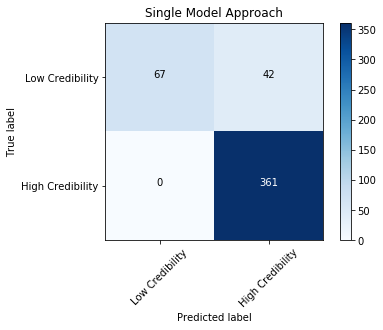
\includegraphics[totalheight=7cm]{images/single-model-performance.png}
	\caption{Performance of single model approach after 10-fold cross validation.}
	\label{fig:SingleModelPerformance}
\end{figure}


The second method, referred to as the ensemble approach, which leverages the best performing models for each criteria (Table \ref{table:EnsembleModel}). The ensemble classifier produced the highest performance results of the three classifiers (Table \ref{table:EnsembleApproach}) with a micro-averaged f1-score of 0.91, an improvement of 7.82\% from its average performance.


\begin{table}[H]
	\centering
	
	\begin{tabular}{|p{4.2cm}|p{5cm}|}
		\hline
		
		\textbf{Criteria} & \textbf{Model}                                                                                                                                                                                                                                                                                                                                                    \\
		\hline                                                                                                                                              
		
		\textbf{Criteria 1}  & SVM + TF-IDF (stopwords removed)  \\
		\hline
		
		\textbf{Criteria 2} & SVM + TF-IDF (stopwords removed)  \\
		\hline
		
		\textbf{Criteria 3} & SVM + BoW (stopwords removed) \\
		\hline
		
		\textbf{Criteria 4} & SVM + BoW (stopwords removed) \\
		\hline
		
		\textbf{Criteria 5}  & SVM + TF-IDF (stopwords removed)  \\
		\hline
		
		\textbf{Criteria 6} & SVM + TF-IDF (stopwords removed)  \\
		\hline
		
		\textbf{Criteria 7} & SVM + BoW (all words) \\
		\hline
		                                                   		
	\end{tabular}
	\caption{Architecture of the ensemble model.}
	\label{table:EnsembleModel}
\end{table}


\begin{table}[H]
	\centering
	\resizebox{\textwidth}{!}{%
	\begin{tabular}{|p{2cm}|p{2cm}|p{2cm}|p{3.5cm}|p{4.5cm}|p{4.5cm}|}
		\hline

		\textbf{Model} & \textbf{Micro-averaged Precision} & \textbf{Micro-averaged Recall} & \textbf{Micro Averaged \newline f1-Score} & \textbf{Average Predicted  Score Differential \newline (Correctly Labelled)}       & \textbf{Average Predicted Score Differential \newline (Incorrectly Labelled)}                                                                                                                                                                                                                                                                                                                                     \\
		\hline                                                                                                                                              
		Ensemble & 0.91 & 0.91 & 0.91 & 0.55 & 2.0 \\
		\hline
		
		
		
	\end{tabular}}
	\caption{Performance of low credibility identification task via an ensemble approach.}
	\label{table:EnsembleApproach}
\end{table}

\begin{figure}[H]
	\centering
	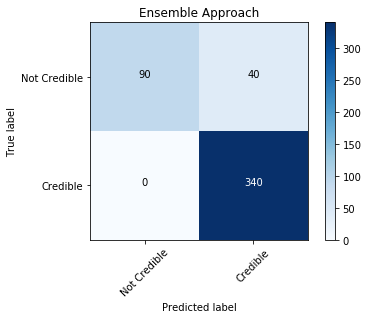
\includegraphics[totalheight=7cm]{images/ensemble-performance.png}
	\caption{Performance of ensemble classifier after 10-fold cross validation.}
	\label{fig:EnsemblePerformance}
\end{figure}

\subsubsection{Binary Classification Approach}
\label{sec:BinaryApproachResults}

\begin{table}[H]
	\centering
		\begin{tabular}{|p{2cm}|p{3.5cm}|p{3.5cm}|p{3.5cm}|}
			\hline
			
			\textbf{Model} & \textbf{Micro-averaged Precision} & \textbf{Micro-averaged Recall} & \textbf{Micro Averaged \newline f1-Score}                                                                                                                                                                                                                                                                                                                                    \\
			\hline                                                                                                                                              
			SVM + \newline TF-IDF \newline (stopwords removed) & 0.61 & 0.61 & 0.61 \\
			\hline
			
			
			
	\end{tabular}
	\caption{Performance of low credibility identification task via a binary classification approach.}
	\label{table:BinaryApproach}
\end{table}

\begin{figure}[H]
	\centering
	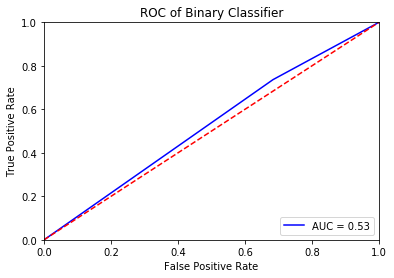
\includegraphics[totalheight=6cm]{images/binary-roc-curve.png}
	\caption{Performance of binary classification approach after 10-fold cross validation.}
	\label{fig:BinaryPerformance}
\end{figure}



\section{Training Time}
\label{sec:TrainingTime}

The training times reported for each model includes the time required to perform the feature-specific preprocessing requirements in addition to the training time of the classifier itself. Information about training times can provide additional support for selecting one approach over others, especially in environments where ongoing training may be needed to update tools used in practice. Since the size and complexity in constructing count-based features such as BoW and TF-IDF (Table \ref{table:CountTrainingTime}), especially when limited to an upper bound, is relatively lower when compared to the construction of statistical-based features such as a language model (Table \ref{table:QRNNTrainingTime}) and relatively smaller than a pre-trained feature such as GloVe (Table \ref{table:PreTrainedTrainingTime}), it is expected that the training times for models that utilise the count-based features are lower.

\begin{table}[H]
	\centering
	
	\begin{tabular}{|p{4.2cm}|p{5cm}|}
		\hline
		
		\textbf{Model} & \textbf{Training Time (seconds)}                                                                                                                                                                                                                                                                                                                                                    \\
		\hline                                                                                                                                              
		
		NB + BoW (all words)  & 5.20  \\
		\hline
		
		NB + BoW \newline (stopwords  removed)  & \textbf{4.86}  \\
		\hline
		
		NB + TF-IDF \newline (all words) & 5.05 \\
		\hline
		
		NB + TF-IDF \newline (stopwords removed) & 5.05 \\
		\hline
		
		SVM + BoW  \newline (all words)  & 5.91  \\
		\hline
		
		SVM + BoW \newline (stopwords removed)  & 4.87  \\
		\hline
		
		SVM + TF-IDF \newline (all words) & 5.35 \\
		\hline
		
		SVM + TF-IDF \newline (stopwords removed) & 5.58 \\
		\hline                                                                                                                                           
		
	\end{tabular}
	\caption{Average training time of models using count-based features.}
	\label{table:CountTrainingTime}
\end{table}



\begin{table}[H]
	\centering
	
	\begin{tabular}{|p{4.2cm}|p{5cm}|}
		\hline
		
		\textbf{Model} & \textbf{Epoch Completion \newline (minutes)}                                                                                                                                                                                                                                                                                                                                                    \\
		\hline                                                                                                                                              
		
		QRNN + General LM  & \textbf{271}  \\
		\hline
		
		QRNN + \newline Fine-tuned LM  & 292  \\
		\hline
		
		
	\end{tabular}
	\caption{Average training time of models using LMs.}
	\label{table:QRNNTrainingTime}
\end{table}

\begin{table}[H]
	\centering
	
	\begin{tabular}{|p{4.2cm}|p{5cm}|}
		\hline
		
		\textbf{Model} & \textbf{Training Time (seconds)}                                                                                                                                                                                                                                                                                                                                                    \\
		\hline                                                                                                                                           
		
		NB + GloVe & 3,628.82 \\
		\hline     
		
		SVM + GloVe & \textbf{3,558.26} \\
		\hline                                                                                                                                        
		
	\end{tabular}
	\caption{Average training time of models using pre-trained GloVe feature.}
	\label{table:PreTrainedTrainingTime}
\end{table}

\section{Model Storage Requirements}
\label{sec:StorageRequirements}

The reported sizes for each of the models are based on the model implmentations in Section \ref{sec:CredibilityClassificationResults}. Due to the model sizes staying relatively unchanged when trained for all criteria (e.g. The size of the NB + BoW (all words) model stayed practically unchanged when trained on each criteria), the aggregated model size of a given model trained on each criteria has been reported. \newline

Models that utilised count-based features (Table \ref{table:CountStorageRequirements}) unsurprisingly had the lowest storage requirements. This is due to its relatively simplistic representation of text in conjunction with the enforced limit on the number of words that are stored. On the other hand, models that utilised the pre-trained GloVe feature (Table \ref{table:PreTrainedStorageRequirements}) has a substantially higher storage requirement due to the feature having a substantially larger vocabulary and higher dimensionality. Whilst this is also explains the storage requirements of models that used LMs (Table \ref{table:LMStorageRequirements}), the LMs used were not trained as extensively as the pre-trained GloVe.

\begin{table}[H]
	\centering
	
	\begin{tabular}{|p{4.2cm}|p{5cm}|}
		\hline
		
		\textbf{Model} & \textbf{Size (MB)}                                                                                                                                                                                                                                                                                                                                                    \\
		\hline                                                                                                                                              
		
		NB + BoW (all words)  & 11.10  \\
		\hline
		
		NB + BoW \newline (stopwords  removed)  & \textbf{11.00} \\
		\hline
		
		NB + TF-IDF \newline (all words) & 13.20 \\
		\hline
		
		NB + TF-IDF \newline (stopwords removed) & 13.20 \\
		\hline
		
		SVM + BoW  (all words)  & 7.91  \\
		\hline
		
		SVM + BoW \newline (stopwords removed)  & \textbf{7.87}  \\
		\hline
		
		SVM + TF-IDF \newline (all words) & 10.00 \\
		\hline
		
		SVM + TF-IDF \newline (stopwords removed) & 7.88 \\
		\hline
		

		
		
	\end{tabular}
	\caption{Aggregated size of count-based models.}
	\label{table:CountStorageRequirements}
\end{table}

\begin{table}[H]
	\centering
	
	\begin{tabular}{|p{4.2cm}|p{5cm}|}
		\hline
		
		\textbf{Model} & \textbf{Size (MB)}                                                                                                                                                                                                                                                                                                                                                    \\
		\hline                                                                                                                                              
		NB + GloVe & 25,410 \\
		\hline
		
		SVM + GloVe & 25,340 \\
		\hline

		
	\end{tabular}
	\caption{Aggregated size of GloVe-based models.}
	\label{table:PreTrainedStorageRequirements}
\end{table}

\begin{table}[H]
	\centering
	
	\begin{tabular}{|p{4.2cm}|p{5cm}|}
		\hline
		
		\textbf{Model} & \textbf{Size (MB)}                                                                                                                                                                                                                                                                                                                                                    \\
		\hline                                                                                                                                              
		QRNN + \newline General LM  & \textbf{3,612.70}  \\
		\hline
		
		QRNN + \newline Fine-tuned LM  & 4,193.35  \\
		\hline
		
		
	\end{tabular}
	\caption{Aggregated size of LM-based models.}
	\label{table:LMStorageRequirements}
\end{table}


\chapter{Discussion}
\label{chap:Discussion}

This chapter examines the feasibility of the implemented and evaluated models in the context of assessing the credibility of vaccine-related articles. The structure of this chapter is as follows. \newline

The reliability of the results reported in Chapter \ref{chap:Results}, is firstly evaluated by examining the consistency of the general trends that emerged from the experiments via the comparison of results from prior literature on text classification tasks (Section \ref{sec:ConsistencyOfResults}). \newline

Feasibility of the models is then evaluated by determining the trade-offs associated between the outcome measures (as identified in Section \ref{sec:Experiments}) and how the priority or importance of each of these measures change depending on the type of application being created (Section \ref{sec:ModelFeasibility}). \newline

Finally, the significance of the obtained results in the context of real-world applications is examined by investigating potential applications of these models based on the advantages and limitations of the top performing models (Section \ref{sec:RealWorldApplication}).

\section{Related Work}
\label{sec:DiscussionRelatedWork}

\subsection{title}

\section{Consistency of Results}
\label{sec:ConsistencyOfResults}

\iffalse
\textbf{Notes about what to talk about:}
\begin{enumerate}[-]
	\item How consistent these results are e.g. no stopwords $>$ having stopwords, ML models $>$ DL models with small datasets with prior literature
	\item Then determine whether the results can be trusted to indicate the feasibility
\end{enumerate}

\textbf{Things to check the consistency on:}
\begin{enumerate}[-]
	\item The performance of SVM $>$ NB (?) $>$ QRNN(DL) for classification tasks with small datasets
	\item The pattern of SVM + TF-IDF $>$ NB + TF-IDF (TFIDF works better with SVMs)
	\item The pattern of NB + GloVe $>$ SVM + GloVe
\end{enumerate}
\fi

Since the classification task performed by the models involve the classification of a novel set of labels (credibility criteria), it is unsuitable to directly compare the performance of the models with any prior work. However, by identifying trends from the reported results, it is possible to determine whether these trends are consistent with the trends found on similar classification tasks from existing literature and thus extrapolate the reliability of the results. \newline

From the reported results, major trends that have been identified are:

\begin{enumerate}
	\item Utilisation of BoW were more successful overall when used in conjunction with NB classifiers rather than SVM classifiers.
	\item Inversely, TF-IDF scores were more effective when paired with SVM classifiers rather than with NB classifiers.
	\item Classical ML models (NB and SVM based models) consistently outperformed DL models (QRNN-based models) on classification tasks with limited training and testing data.
	\item The process of fine-tuning a LM in order to learn task specific features consistently improved the model's performance.
\end{enumerate}

The sentiment classification task using the subjectivity dataset \cite{Pang2004} evaluated by Wang et al. \cite{Wang2012} and the product-review classification task performed by Pranckevičius et al. \cite{PRANCKEVICIUS2017} attained results that aligned with the first major trend described above. Both works presented results that showed better performance when using BoW with a NB classifier over a SVM classifier. The work conducted by Wang et al. involved evaluating a linear SVM and multinomial NB classifier in combination with a unigram BoW model to perform a binary sentiment analysis task on movie reviews (`thumbs up', `thumbs down') \cite{Pang2004}. Similarly, Pranckevicius et al., performed a multi-class classification task, that aimed to predict the resulting product review score (ranging from 1 to 5) from reviews on Amazon \cite{PRANCKEVICIUS2017}. For the sentiment analysis task, the NB-based model had an improved performance of 5.5\% over the SVM-based model and the product-review classification task reported an improvement of 2.4\% by the NB-based model over the SVM-based model. These results align with the measurements obtained from the classification experiment reported in Section \ref{sec:CredibilityClassificationResults} which showed the NB-based model having a higher average performance by a margin of 0.25\%. \newline

The diminishing difference in performance between the NB-based models and the SVM-based models relative to the aforementioned literature may have a relation to the increasing number of classes being classified in these tasks. This is somewhat supported by the results obtained by Hassan et al. \cite{Hassan} who evaluated NB and SVM based models using the 20 Newsgroups dataset \cite{Mitchell} which consists of 20 classes where the baseline performance of the SVM-based models outperformed the NB-based models by 25\%. This however does not conclusively explain the diminishing difference as Hassan et al. utilised domain-specific information extracted from as features for the construction of their models. The common factor in regards to the construction of the models resides within the preprocessing phase where only the stopwords of the text were removed. \newline


\textit{The following paragraph discusses the consistency of TFIDF working better with SVMs rather than NBs}

\textit{[-----------------]}

\textit{The following paragraph discusses the consistencty of ML models outperforming DL models for text classification tasks with limited data}

\textit{[-----------------]}

\textit{The following paragraph discusses the consistent results of fine-tuned LMs outperforming general-domain LMs}

While the performance of the QRNN-based models was lower than what was initially expected, this can be theorised to be due to the relatively low number of vaccine-related training samples utilised during the training of the fine-tuned LM. When compared to the work conducted by Howard et al. \cite{Howard2018} for the task of question classification, the number of training samples used to construct the discriminative fine-tuned LM was 5,500 which only improved the model's performance by 0.3\%. 

\section{Model Feasibility}
\label{sec:ModelFeasibility}
Notes about what to talk about:
\begin{enumerate}[-]
	\item Discuss the trade-offs between optimising the performance, training time and storage requirements and the factors that affect these measures. 
	\item What it means to be feasible e.g. it is application dependent and depending on the application some factors might be more important than others such as having a higher true negative rate can be alright for some tasks and that having a high false positive rate is usually always bad.
\end{enumerate}

\section{Real World Applications}
\label{sec:RealWorldApplication}
\textit{This is where I'll be talking about the performance of constructing and testing the low credibility classifiers}
So once the credibility of the results have been verified and also what the feasibility of a model entails, I can then talk about:

\begin{enumerate}[-]
	\item Possible applications of the models e.g. web browser extension, twitter bot, article filtering system and the differing priorities they have on the for outcome measures (accuracy, training time and storage requirements)
\end{enumerate}

\chapter{Conclusions and Future Work}
\label{chap:Conclusions}
This section will be completed after the fulfilment of the proposed work detailed in Section \ref{chap:ProposedWork}

\section{Future Work}
\label{FutureWork}

\section{Conclusions}
\label{sec:ConclusionsConclusions}



\clearemptydoublepage

%\phantomsection \addcontentsline{toc}{chapter}{Index}
% \renewcommand{\baselinestretch}{1} \small \normalsize
% \printindex

\appendix
\chapter{Exmaple}
\section{Overview}
This is an example entry in the appendix



%\input{Bibliography/biblio3}
\bibliographystyle{IEEEtranS}
%\bibliographystyle{acm}
\bibliography{my_reference}
%\bibliography{Bibliography/biblio4}


\end{document}
